We will now compare the standard and hierarchical implementation against a real data set.
A common application of networks is in caching queries. Thus, we will use AOL data, which is a collection of query data \cite{AOL}.
We will extract out all the unique queries. We will randomly select 700

\begin{center}
    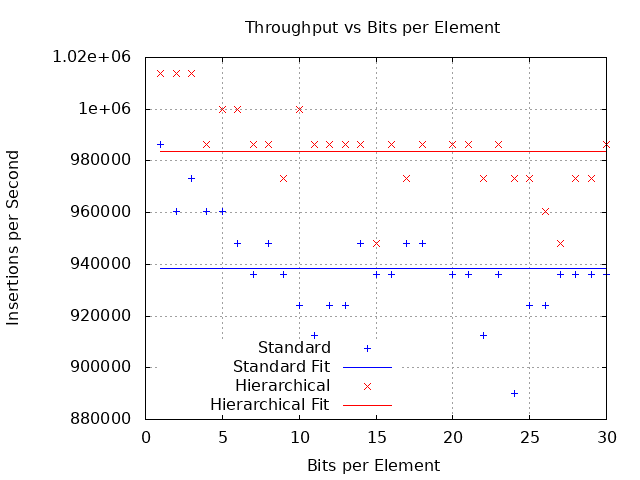
\includegraphics[width=14cm]{aol_thru.png}
\end{center}

\begin{center}
    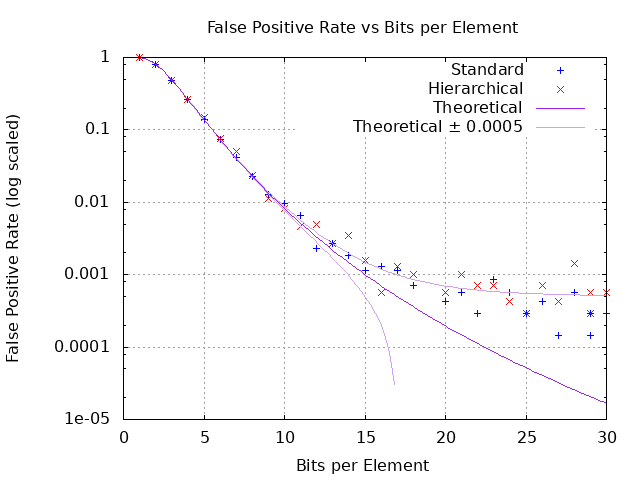
\includegraphics[width=14cm]{aol_fp.png}
\end{center}